\documentclass[tikz,border=3.14mm]{standalone}
\usepackage{amsmath, amssymb}
\usetikzlibrary{shapes.geometric, arrows.meta, bending}

\begin{document}

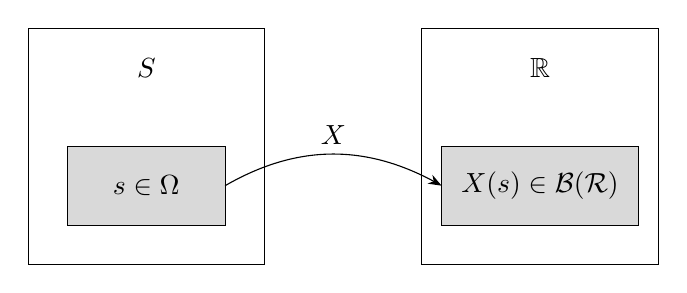
\begin{tikzpicture}[>=Stealth]

% Draw the first box and label it as the preimage
\draw (0,0) rectangle (3,3);
\node at (1.5,2.5) {$S$};
\draw[fill=gray!30] (0.5,0.5) rectangle (2.5,1.5);
\node at (1.5,1) {\( s \in \Omega \)};

% Draw the second box and label it as the image
\draw (5,0) rectangle (8,3);
\node at (6.5,2.5) {$\mathbb R$};
\draw[fill=gray!30] (5.25,0.5) rectangle (7.75,1.5);
\node at (6.5,1) {\( X(s) \in \mathcal B(\mathcal R)\)};

% Draw a curved arrow from subset A of the preimage to the subset f(A) of the image
\draw[->] (2.5,1) to[out=30,in=150] node[midway, above] {\( X \)} (5.25,1);

\end{tikzpicture}

\end{document}
